\documentclass[compress,10pt,aspectratio=169]{beamer}
\usetheme[customnumbering]{onera}

\usepackage{amsmath,amsfonts,graphicx}
\usepackage{pifont}
\usepackage{etoolbox}
\usepackage{multicol}
\usepackage{anyfontsize}
\usepackage{multirow}
\usepackage{hyperref}
\usepackage{amsmath}
\usepackage{fancybox}
\usepackage{colortbl}
\usepackage{tcolorbox}
%\setlength{\columnseprule}{1pt}
%\def\columnseprulecolor{\color{blue}}
\usepackage{minted} % syntax coloring.
\usepackage{algorithm2e}
\setminted{encoding=utf-8, autogobble}
\usemintedstyle{xcode}
\AtBeginEnvironment{minted}{\fontsize{7}{7}\selectfont}

%\usepackage{dsfont}
\usepackage{ifdraft}
\ifdraft{
  \usepackage{fancyvrb}
  \DefineVerbatimEnvironment{cppcode}{Verbatim}{}
}{
\newminted{cpp}{}
}
\usepackage{hyperref}
\usetikzlibrary{shadows, arrows, arrows.meta, decorations.pathmorphing, fadings, shapes.arrows, positioning, calc, shapes, fit, matrix,math, tikzmark, patterns}

\definecolor{lightblue}{RGB}{0,200,255} 
\definecolor{paper}{RGB}{255,247,197}
\definecolor{ocre}{RGB}{243,102,25} % Define the orange color used for highlighting throughout the book
\definecolor{BurntOrange}{RGB}{238,154,0}
\definecolor{darkorange}{RGB}{119, 77, 0}
\definecolor{OliveGreen}{RGB}{188,238,104}
\definecolor{DarkGreen}{RGB}{0,128,0}
\definecolor{BrickRed}{RGB}{238,44,44}
\definecolor{Tan}{RGB}{210,180,140}
\definecolor{Aquamarine}{RGB}{127,255,212}
\definecolor{NavyBlue}{RGB}{0,64,128}
\definecolor{DarkYellow}{RGB}{192,192,0}
\definecolor{Yellow}{RGB}{255,255,0}
\definecolor{navyblue}{rgb}{0.1,0.2,0.7}

\tikzset{square matrix/.style={
    matrix of nodes,
    column sep=-\pgflinewidth, row sep=-\pgflinewidth,
    nodes={draw,
      minimum height=#1,
      anchor=center,
      text width=#1,
      align=center,
      inner sep=0pt
    },
  },
  square matrix/.default=1.2cm
}

\setbeamercovered{transparent}
\newcommand{\compute}[1]{\pgfmathparse{#1}\pgfmathresult}

\title[Parallel programming\hspace{2em}]{Domain decomposition}
\subtitle{Theory and implementation}
\author[X. JUVIGNY]{Xavier JUVIGNY, SN2A, DAAA, ONERA\\ \href{mailto:xavier.juvigny@onera.fr}{\texttt{xavier.juvigny@onera.fr}} }
\date[01/08/2023]{Course Parallel Programming\\- January 8th 2023 -}
\institute{\inst{1}ONERA,\inst{2}DAAA}

\AtBeginSection[]{
  \begin{frame}{Overview}
  \begin{multicols}{2}
  \small \tableofcontents[currentsection, hideallsubsections]
  \end{multicols}
  \end{frame} 
}


\begin{document}

\MakeTitlePage

\begin{frame}
\frametitle{Table of contents}
\begin{multicols}{2}
\tableofcontents[hideallsubsections]
\end{multicols}
\end{frame}

\section{Generalities}

\begin{frame}[fragile]{Main ideas}
    \scriptsize

    \begin{block}{\small Principles}
        \begin{itemize}
            \item Split a finite computing domain $\Omega$ (picture, spatial domain, \dots) in some sub-domains $\Omega_{i}$;
            \item Apply a local method on each subdomains;
            \item Apply if necessary a global method to find the global result on $\Omega$;
            \item The last two steps can be in a direct or iterative method.
        \end{itemize}
    \end{block}

    \begin{exampleblock}{\small Example : JPEG 2000 compression (Wikipedia)}
        \begin{itemize}
            \item Color components transformation (RGB to YUV);
            \item Image is split into tiles (subdomains);
            \item Wavelet transformation of each tile;
            \item Quantization of wavelet transformation of each tile.
        \end{itemize}
    \end{exampleblock}
\end{frame}

\begin{frame}[fragile]{Classification of domain decomposition methods}
    \scriptsize

    \begin{block}{\small Types of domain decomposition methods}
        \begin{itemize}
            \item \textcolor{blue}{\bf Overlapping domain decomposition methods} : The sub-domains share common cells (pixels, elements, \dots);
            \item \textcolor{blue}{\bf Non Overlapping domain decomposition methods} : The sub-domains don't share common cells (pixels, elements, \dots).
        \end{itemize}
    \end{block}

    \begin{multicols}{2}
    \begin{alertblock}{\small Non overlapping domain decomposition methods}
        Splitting $\Omega$ in $n$ subdomains $\Omega_{i}, i=1,\cdots,n$ verifying 
        \begin{enumerate}
            \item $\Omega_{i}\neq \emptyset, i=1,\cdots,n$;
            \item $\cup_{i=1}^{n} \overline{\Omega_{i}} = \overline{\Omega}$;
            \item $\Omega_{i} \cap \Omega_{j} = \emptyset; i\neq j$;
            \item $\overline{\Omega_{i}} \cap \overline{\Omega_{j}} \neq \emptyset; i\neq j$.
        \end{enumerate}
    \end{alertblock}

    \begin{figure}
        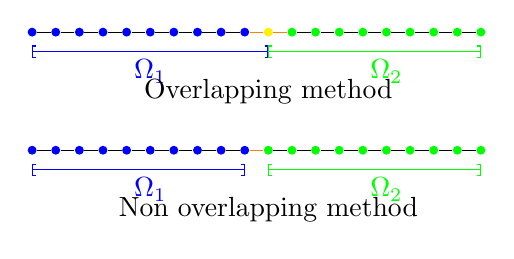
\begin{tikzpicture}
            \foreach \x in { 0,1, ..., 9}
            {
                \node[fill=blue,circle,inner sep=0.4mm] (A\x) at (0.3*\x,0) {};
            }
            \draw (A0) -- (A1);
            \draw (A1) -- (A2);
            \draw (A2) -- (A3);
            \draw (A3) -- (A4);
            \draw (A4) -- (A5);
            \draw (A5) -- (A6);
            \draw (A6) -- (A7);
            \draw (A7) -- (A8);
            \draw (A8) -- (A9);

            \node[fill=yellow,circle,inner sep=0.4mm] (A10) at (3,0) {};

            \foreach \x in { 11,12, ...,19}
            {
                \node[fill=green,circle,inner sep=0.4mm] (A\x) at (0.3*\x,0) {};
            }
            \draw (A11) -- (A12);
            \draw (A12) -- (A13);
            \draw (A13) -- (A14);
            \draw (A14) -- (A15);
            \draw (A15) -- (A16);
            \draw (A16) -- (A17);
            \draw (A17) -- (A18);
            \draw (A18) -- (A19);

            \draw[color=orange] (A9)  -- (A10);
            \draw[color=orange] (A10) -- (A11);

            %\node at (1.5, 0.5) {\textcolor{blue}{$\Omega_{1}$}};
            %\draw[arrows = {-Bracket[reversed,line cap=butt]},color=blue] (0,0.25) -- (3,0.25);
            %\node at (4.5, 0.5) {\textcolor{green}{$\Omega_{2}$}};
            %\draw[arrows = {-Bracket[reversed,line cap=butt]},color=green] (5.7,0.25) -- (3,0.25);
            %\node at (3.0, 0.5) {\textcolor{red}{$\Omega_{3}$}};

            \node at (1.5, -0.5) {\textcolor{blue}{$\Omega_{1}$}};
            \draw[arrows = {Bracket[line cap=butt]-Bracket[line cap=butt]},color=blue] (0,-0.25) -- (3,-0.25);
            \node at (4.5, -0.5) {\textcolor{green}{$\Omega_{2}$}};
            \draw[arrows = {Bracket[line cap=butt]-Bracket[line cap=butt]},color=green] (5.7,-0.25) -- (3,-0.25);

            \node at (3,-0.75) {Overlapping method};
            %%%%%%%%%%%%%%%%%%%%%%%%%%%%%%%%%%%%%%%%%%%%%%%%%%%%%%%%%%%%%
            \foreach \x in { 0,1, ..., 9}
            {
                \node[fill=blue,circle,inner sep=0.4mm] (B\x) at (0.3*\x,-1.5) {};
            }
            \draw (B0) -- (B1);
            \draw (B1) -- (B2);
            \draw (B2) -- (B3);
            \draw (B3) -- (B4);
            \draw (B4) -- (B5);
            \draw (B5) -- (B6);
            \draw (B6) -- (B7);
            \draw (B7) -- (B8);
            \draw (B8) -- (B9);

            \foreach \x in { 10,11,12, ...,19}
            {
                \node[fill=green,circle,inner sep=0.4mm] (B\x) at (0.3*\x,-1.5) {};
            }
            \draw (B10) -- (B11);
            \draw (B11) -- (B12);
            \draw (B12) -- (B13);
            \draw (B13) -- (B14);
            \draw (B14) -- (B15);
            \draw (B15) -- (B16);
            \draw (B16) -- (B17);
            \draw (B17) -- (B18);
            \draw (B18) -- (B19);

            \draw[color=orange] (B9)  -- (B10);

            \node at (1.5, -2.0) {\textcolor{blue}{$\Omega_{1}$}};
            \draw[arrows = {Bracket[line cap=butt]-Bracket[line cap=butt]},color=blue] (0,-1.75) -- (2.7,-1.75);
            \node at (4.5, -2.0) {\textcolor{green}{$\Omega_{2}$}};
            \draw[arrows = {Bracket[line cap=butt]-Bracket[line cap=butt]},color=green] (5.7,-1.75) -- (3.,-1.75);

            \node at (3,-2.25) {Non overlapping method};

        \end{tikzpicture}
    \end{figure}
    \end{multicols}
\end{frame}

\begin{frame}[fragile]{How to split a computing domain ?}
    \scriptsize
    Let $\Omega$ be a rectangular area in $\mathbb{R}^{2}$.

    Some types of splitting :
    \begin{itemize}
        \item One direction splitting : Easy to care, but not efficient for communications;
        \item Alternate direction      : Split in two, four or height subdomains the initial domain $\Omega$ and iterate the splitting for subdomains; Harder to care for but more efficient for parallelization and communication;
        \item Adaptive splitting : Anyway, for parallel efficiency, better to split in the direction where we have a minimal number of cells.
    \end{itemize}

    \begin{figure}
        \begin{tikzpicture}
            \draw[fill=yellow,draw] (-4,-2) -- (-2,-2) -- (-2, 1) -- (-4,1) -- cycle;
            \draw[fill=yellow,draw] (-4,-2) grid[xstep=0.1,ystep=0.1] (-2, 1);
            \draw[fill=yellow,draw] (2,-2) -- (0,-2) -- (0, 1) -- (2,1) -- cycle;
            \draw[fill=yellow,draw] (2,-2) grid[xstep=0.1,ystep=0.1] (0, 1);
            \draw[fill=yellow,draw] (4,-2) -- (6,-2) -- (6, 1) -- (4,1) -- cycle;
            \draw[fill=yellow,draw] (4,-2) grid[xstep=0.1,ystep=0.1] (6, 1);

            \only<4>{\draw[color=green,draw,thick] (-3.7,-2) -- (-3.7,1);}
            \only<4>{\draw[color=green,draw,thick] (-3.2,-2) -- (-3.2,1);}
            \only<4>{\draw[color=green,draw,thick] (-2.7,-2) -- (-2.7,1);}
            \only<4>{\draw[color=green,draw,thick] (-2.2,-2) -- (-2.2,1);}
            \only<4>{\draw[color=green,draw,thick] (1.5,-2) -- (1.5,1);}
            \only<4>{\draw[color=green,draw,thick] (0.5,-2) -- (0.5,1);}
            \only<4>{\draw[color=green,draw,thick] (4,-1.2) -- (6,-1.2);}
            \only<4>{\draw[color=green,draw,thick] (4,0.2) -- (6,0.2);}

            \only<3-4>{\draw[color=blue,draw,thick] (-3.5,-2) -- (-3.5,1);}
            \only<3-4>{\draw[color=blue,draw,thick] (-2.5,-2) -- (-2.5,1);}
            \only<3-4>{\draw[color=blue,draw,thick] (2,-0.5) -- (0,-0.5);}
            \only<3-4>{\draw[color=blue,draw,thick] (5,-2) -- (5,1);}

            \only<2-4>{\draw[color=red,draw,thick] (-3,-2) -- (-3,1);}
            \only<2-4>{\draw[color=red,draw,thick] (1,-2) -- (1,1);}
            \only<2-4>{\draw[color=red,draw,thick] (4,-0.5) -- (6,-0.5);}

            \node at (-3,-2.5) {\scriptsize One direction splitting};
            \node at (+1,-2.5) {\scriptsize Alternate direction splitting};
            \node at (+5,-2.5) {\scriptsize Adaptive direction splitting};
        \end{tikzpicture}
    \end{figure}
\end{frame}

\begin{frame}[fragile]{Domain decomposition for unstructured mesh}
    \scriptsize

    \begin{multicols}{2}
    \begin{block}{\small unstructured mesh}
        \begin{itemize}
            \item Mesh where cells can't be located with (multi-)indices;
            \item For example, a triangular mesh
        \end{itemize}
    \end{block}

    \begin{exampleblock}{\small How to split an unstructured mesh?}
        \begin{itemize}
            \item Minimize the size of the interfaces between sub-domains;
            \item Optimal minimization is a NP-problem. 
            \item Use some approximations or heuristics
            \item Some libraries exist for graph partitioning :
            \begin{itemize}
                \item {\scriptsize scotch (Inria);}
                \item {\scriptsize metis (Karypis Lab)};
            \end{itemize}
        \end{itemize}
    \end{exampleblock}

    \begin{figure}[h]
    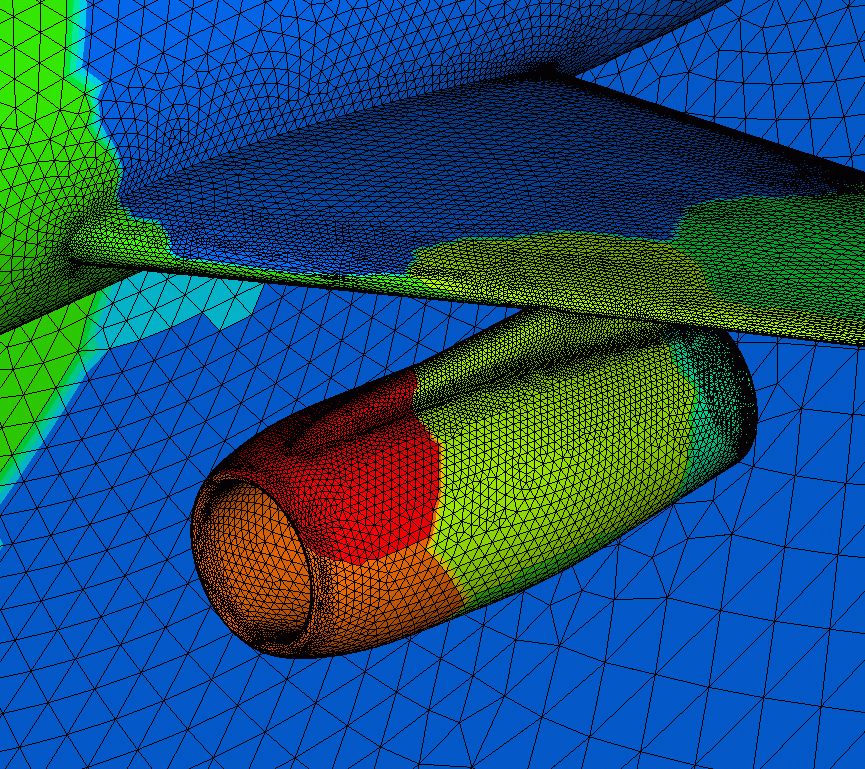
\includegraphics[width=0.40\textwidth]{../Images/grid_decomposition.png}
    \caption{Fun 3D (NASA)}
    \end{figure}
\end{multicols}
\end{frame}

\section{Overlapping domain decomposition methods}



\subsection{Explicit methods}

\begin{frame}[fragile]{Baseline problem}
\scriptsize

\begin{multicols}{2}
\begin{block}{\small Laplacian filter on a gray-scale image}
    \begin{itemize}
        \item A pixel $p_{i,j}$ located by i and j indices on grid
        \item $v_{i,j}$ is the intensity of the pixel $p_{i,j}$;
        \item Discrete Laplacian scheme\\
        $u_{i,j} = v_{i-1,j}+v_{i+1,j}+v_{i,j-1}+v_{i,j+1}-4v_{ij}$
        \item Consider pixel out of the image as black ($=0$)
    \end{itemize}
\end{block}

\begin{figure}
    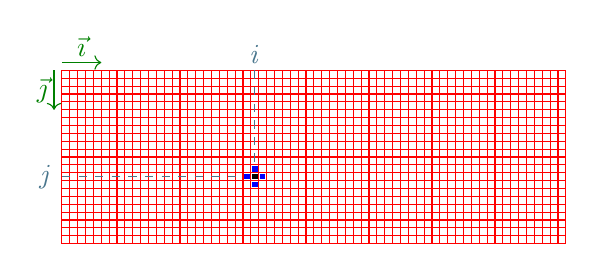
\begin{tikzpicture}
    \draw[color=red] (0,1) grid[step=0.1] (6.4001,3.2001    );        
    \node[fill=black,minimum size=0.1, inner sep=1.0] at (2.45,1.85) {};
    \node[fill=blue,minimum size=0.1, inner sep=1.0] at (2.35,1.85) {};
    \node[fill=blue,minimum size=0.1, inner sep=1.0] at (2.55,1.85) {};
    \node[fill=blue,minimum size=0.1, inner sep=1.0] at (2.45,1.75) {};
    \node[fill=blue,minimum size=0.1, inner sep=1.0] at (2.45,1.95) {};
    \draw[color=DarkGreen, ->] (0,3.3) -- (0.5,3.3) node at (0.25, 3.5) {$\vec{\imath}$};
    \draw[color=DarkGreen, ->] (-0.1,3.2) -- (-0.1,2.7) node at (-0.25,2.95) {$\vec{\jmath}$};
    \draw[color=cyan!50!black, dashed] (2.45, 3.2001) -- (2.45, 2.0) node at (2.45,3.4) {$\mathit{i}$};
    \draw[color=cyan!50!black, dashed] (0, 1.85) -- (2.3, 1.85) node at (-0.2,1.85) {$\mathit{j}$};
    \end{tikzpicture}
\end{figure}
\end{multicols}

\begin{multicols}{2}
\begin{minipage}{0.45\textwidth}
  \begin{figure}
    
\includegraphics[width=0.35\textwidth]{../Images/ned.png}
    \caption{\scriptsize Before filter}
  \end{figure}
\end{minipage}
\begin{minipage}{0.45\textwidth}
  \begin{figure}
    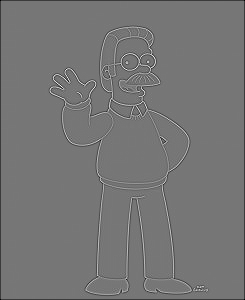
\includegraphics[width=0.35\textwidth]{../Images/lapl_ned.png}
    \caption{\scriptsize After filter}
  \end{figure}
\end{minipage}
\end{multicols}
\end{frame}

\begin{frame}[fragile]{Ghost cells}
  \scriptsize
  \begin{multicols}{2}
  \begin{block}{\small Parallelization of the laplacian filter}
    \begin{itemize}
    \item Apply decomposition domain on image domain;
    \item But need nearby pixels (right, left, above, bottom);
    \item Add a layer of image pixels in each direction
    \item These pixels are named \textsl{ghost cells};
    \item For sub-domain which contains boundary condition,\\
      fill ghost cells with adequate values (0 for laplacian filter).
    \item Application of laplacian filter is a nearly embarassingly parallel algorithm
    \item One must rebuild the complete filtered image after application \\ of laplacian filter.
    \end{itemize}
  \end{block}

  \begin{alertblock}{\small Remarks}
    \begin{itemize}
    \item \alert{If possible}, each process reads his part of the image;
    \item Better to use communicator splitting and global communication than point to point communication
      when rebuilding complete image.
    \end{itemize}
  \end{alertblock}
  
  \begin{center}
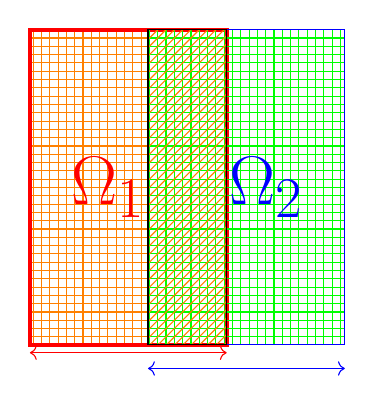
\begin{tikzpicture}
  \draw[color=red, ultra thick, pattern=grid, pattern color=orange] (-2,-2) rectangle (0.5,2);
  \draw[color=blue, pattern=grid, pattern color=green] (-0.5,-2.) rectangle (2,2.);
  \draw[pattern color=orange, pattern = north east lines] (-0.5,-2.) rectangle (0.5,2.);
  \node[color=red] at (-1,0) {\Huge \bf $\Omega_{1}$};
  \node[color=blue] at (1,0) {\Huge \bf $\Omega_{2}$};
  \draw[<->, color=red] (-2,-2.1) -- (0.5,-2.1);
  \draw[<->, color=blue] (-0.5,-2.3) -- (2,-2.3);
  %\draw[ultra thick, loosely dotted,color=orange] (0,0) circle (2cm);
\end{tikzpicture}
\end{center}
\end{multicols}
\end{frame}

\subsection{Implicit methods}

\begin{frame}[fragile]{Inpainting algorithm}
  \scriptsize
  \begin{block}{\small Definition}
    Inverse operation of laplacian filter. From filtered image, rebuild the original image.

    \begin{itemize}
    \item It's an inverse laplacian problem;
    \item This problem has a unique solution, thanks to the boundary (Dirichlet) condition (fixed value 0 out of the image);
    \item Inpainting is a research domain to achieve real-time decoding for 4K colour images of size $3840\times 2160$ pixels for TV applications using GPGPU (Domain decomposition algorithms for real-time homogeneous diffusion inpainting in 4k, Niklas Kämper and Joachim Weickert, 14 February 2022).
    \item Symmetric definite positive linear system to solve;
    \item The left hand side matrix is the laplacian filter !
    \item Use some iterative or direct solver (conjugate gradient or sparse LU algorithm for example).
    \end{itemize}
  \end{block}
\end{frame}

\begin{frame}[fragile]{Parallel conjugate gradient algorithm}
  \scriptsize
  \begin{multicols}{2}
  \begin{exampleblock}{\small Conjugate gradient algorithm}
    \begin{algorithm}[H]
      $p_{0} = r_{0} = b-A.x_{0}$\;
      $k=0$\;
      \While{$\|r_{k}\|>\varepsilon$}{
        $\alpha_{k} = \frac{\|r_{k}\|^{2}}{p_{k}^{T}Ap_{k}}$\;
        $x_{k+1}=x_{k} + \alpha_{k}p_{k}$\;
        $r_{k+1}=r_{k} - \alpha_{k}Ap_{k}$\;
        \If{$\|r_{k+1}\|<\varepsilon$}{
          exit loop\;
        }
        $\beta_{k} = \frac{\|r_{k+1}\|^{2}}{\|r_{k}\|^{2}}$\;
        $p_{k+1} = r_{k+1} + \beta_{k}p_{k}$\;
        $k \leftarrow k+1$\;
      }
      return $x_{k+1}$ as the result\;
    \end{algorithm}
  \end{exampleblock}

  \begin{itemize}
  \item Usually, if no smart $x_{0}$ can be chosen, one takes null vector as $x_{0}$;
  \item Very slow to converge $\Rightarrow$ use a local preconditioner;
  \item Same splitting of the image for parallel implementation;
  \item For parallel implementation, processes must exchanges values to update ghost cells value for each iteration of conjugate gradient;
    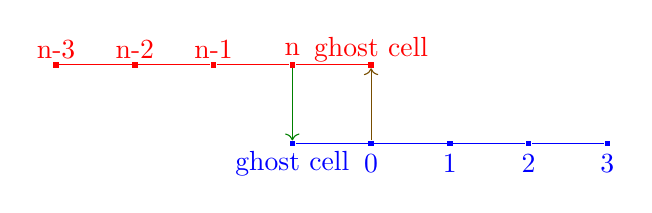
\begin{tikzpicture}
      \node[fill=red,inner sep=1.0] (P0) at (0,0){};
      \node[red] at (0,0.2){n-3};
      \node[fill=blue,inner sep=1.0] (Q0) at (3,-1){};
      \node[blue] at (3,-1.25){ghost cell};
      \foreach \x [evaluate=\x as \y using {int(\x-1)}] in {1,2,3,4} {
        \node[fill=red,inner sep=1.0] (P\x) at (\x,0){};
        \draw[red] (P\y) -- (P\x);
        \node[fill=blue,inner sep=1.0] (Q\x) at (\x+3,-1){};
        \draw[blue] (Q\y) -- (Q\x);
        \node[blue] at (\x+3,-1.25){\y};
      }
      \node[red] at (1,0.2){n-2};
      \node[red] at (2,0.2){n-1};
      \node[red] at (3,0.2){n};
      \node[red] at (4,0.2){ghost cell};
      \draw[DarkGreen, ->] (P3) -- (Q0);
      \draw[darkorange, ->] (Q1) -- (P4);
    \end{tikzpicture}
  \item Computing dot product or norm of vector needs global reduction.
  \end{itemize}
  \end{multicols}
\end{frame}

\begin{frame}[fragile]{Efficiency of parallel conjugate gradient algorithm}
  \scriptsize
  \begin{block}{Efficiency}
    Given an image with resolution $W\times H$ pixels.\\
    Let $N = W \times H$ be the number of pixels contained in the image. So, per iteration of conjugate gradient :
    \begin{itemize}
    \item About $5\frac{N}{nbp}$ additions and multiplications
    \item About $\displaystyle \frac{2}{\sqrt{\mbox{nbp}}}\left(W + H\right)$ data to send and receive when using alternating
          direction splitting, or $2\min\left(W,H\right)$ data to send and receive when using one direction splitting.
    \item For adaptative direction splitting, one has less than the best of formulae above.
    \end{itemize}
  \end{block}
\end{frame}

\begin{frame}{Schwarz's Domain Decomposition Method}
  \scriptsize
  \begin{block}{\small Presentation of the method}
    \begin{itemize}
      \item Introduced by Schwarz (1869) to prove existence \& uniqueness of Poisson problem, dividing domain
            in simpler geometry
      \item With the advent of digital computers, this method acquired a pratical interest as in iterative solver
      \item Parallel computers make it suited to this architecture.
    \end{itemize}
  \end{block}

  \begin{exampleblock}{The algorithm on two subdomains}
    Let $\Omega$ be a domain in $\mathbb{R}^{n}$ and $\Omega_{1},\Omega_{2}$ two subdomains as $\Omega_{i}\subset \Omega$,
    $\Omega_{1}\cup \Omega_{2} = \Omega$ and $\Omega_{1}\cap \Omega_{2} \neq \emptyset$. The Schwarz method to solve the
    Poisson problem on $\Omega$ is an iterative method :
    \begin{itemize}
      \item Start with initial solutions $u^{(0)}_{1},u^{(0)}_{2}$ on respectively $\Omega_{1}, \Omega_{2}$;
      \item To compute $u^{(n+1)}_{1}, u^{(n+1)}_{2}$ from $u^{(n)}_{1}, u^{(n)}_{2}$, solve :
      \vspace*{-5mm}
      \begin{multicols}{2}
        \[
          \left\{
            \begin{array}{lcl}
              -\Delta u_{1}^{(n+1)} & = & f \mbox{ in }\Omega_{1}\\
              u_{1}^{(n+1)} & = & 0 \mbox{ on } \partial\Omega_{1} \cap \partial \Omega \\
              u_{1}^{(n+1)} & = & u_{2}^{(n)} \mbox{ on } \partial\Omega_{1} \cap  \overline{\Omega_{2}}
            \end{array}
          \right.
        \]

        \[
          \left\{
            \begin{array}{lcl}
              -\Delta u_{2}^{(n+1)} & = & f \mbox{ in }\Omega_{2}\\
              u_{2}^{(n+1)} & = & 0 \mbox{ on } \partial\Omega_{2} \cap \partial\Omega \\
              u_{2}^{(n+1)} & = & u_{1}^{(n)} \mbox{ on } \partial\Omega_{2} \cap \overline{\Omega_{1}}
            \end{array}
          \right.
        \]
      \end{multicols}
    \end{itemize}
  \end{exampleblock}
\end{frame}

\begin{frame}[fragile]{Practical implementation}
  \scriptsize
  \begin{multicols}{2}
  \begin{block}{\small Tips}
    \begin{itemize}
      \item Using ghostcells to update fixed values on\\ $\partial\Omega_{i} \cap \Omega_{3-i}, i\in\{1,2\}$
      \item Solve local values with direct or iterative method\\ (GC by example)
      \item Direct solve is faster. Factorize local matrix before\\ Schwarz iterative method;
      \item Stop criterion : stop Schwarz iterations when \\
      $\displaystyle\max_{i=1,2}\left(\|u_{i}^{(n+1)} - u_{i}^{(n)}\|\right) < \varepsilon$
      \item Using more subdomains is straightforward !
      \item But when more subdomains are used, slower is the convergence.
      \item Some methods exist to speed-up the convergence of the\\ method (coupling with multigrid method for example)
    \end{itemize}
  \end{block}

  \begin{exampleblock}{\small Pratical algorithm}
    \begin{algorithm}[H]
      Choose $u_{i}$\;
      $u_{i}^{(old)} \leftarrow 0$\;
      \While{reduce($\|u_{i} - u_{i}^{(old)}\|,\mbox{max}) < \varepsilon$} {
          $u_{i}^{(old)} \leftarrow u_{i}$\;
          update ghost cells for $u_{i}$\;
          Solve($u_{i}, f$) using ghostcells as boundary conditions\;
      }
    \end{algorithm}
  \end{exampleblock}
\end{multicols}
\end{frame}

\begin{frame}[fragile]{Properties of Schwarz's algorithm}
\scriptsize
\begin{block}{\small Properties}
  \begin{itemize}
    \item Some mathematical theorems show than the algorithm converges
    \item Greater is the overlapping between domains, faster is the convergence of the algorithm
    \item But solving local problems is slower
    \item And more memory is consumed
  \end{itemize}
\end{block}  

\begin{exampleblock}{\small Complexity analysis}
  \begin{itemize}
    \item For each iteration, computing complexity is the complexity to solve the linear system issued from Laplacian operator;
    \item Beware, Gradient Conjugate algorithm will be purely local if used;
    \item For communication, for each iteration of Schwarz's algorithm, updating ghostcells needs communication as :
    $\displaystyle \frac{2}{\sqrt{\mbox{nbp}}}\left(W + H\right)$ data to send and receive when using alternating
    direction splitting, or $2\min\left(W,H\right)$ data to send and receive when using one direction splitting.
  \item For adaptative direction splitting, one has less than the best of formulae above.
  \end{itemize}
\end{exampleblock}
\end{frame}

\section{Non overlapping domain decomposition methods}

\begin{frame}[fragile]{Non overlapping methods}
  \scriptsize
  \begin{block}{\small Non overlapping domain decomposition}
    \begin{itemize}
      \item $\left\{\Omega_{i}\right\}_{i=1,\cdots,n}$ is a non overlapping decomposition method of $\Omega$ if :
      \begin{itemize}
        \item {\scriptsize $\Omega_{i} \bigcap \Omega_{j} = \emptyset$ where $i\neq j$}
        \item {\scriptsize $\displaystyle \bigcup_{i=1,\cdots,n}\overline{\Omega_{i}} = \overline{\Omega}$}
        \item {\scriptsize $\overline{\Omega_{i}} \bigcap \overline{\Omega_{j}} \neq \emptyset$}
      \end{itemize}
      \item Example : $\Omega = ]0;1[ \Rightarrow \Omega_{1} = ]0;\frac{1}{2}[ \mbox{ and } \Omega_{2} = ]\frac{1}{2};1[$
    \end{itemize}
  \end{block}

  \begin{exampleblock}{\small Non overlapping methods for image}
    \begin{itemize}
      \item In fact, to split an image in two sub-images, we must share a common interface, i.e a simple row (or column) of pixels
      \item This common interface can be a third sub-images or the boundary condition of both sub-images.
    \end{itemize}
  \end{exampleblock}
\end{frame}

\subsection{Explicit methods}

\begin{frame}{Primal schur factorization}
  \scriptsize
  \begin{block}{Principle with two sub-domains and an interface}
    \begin{multicols}{2}
    \begin{figure}[h]
      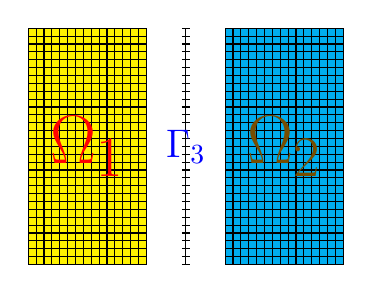
\begin{tikzpicture}
        \draw[fill=yellow,draw] (-2,-2) -- (-0.5,-2) -- (-0.5, 1) -- (-2,1) -- cycle;
        \draw[fill=yellow,draw] (-2,-2) grid[xstep=0.1,ystep=0.1] (-0.5, 1);
        \node at (-1.25, -0.5) {\textcolor{red}{\Huge $\Omega_{1}$}};

        \draw[fill=yellow,draw] (0,-2) --  (0,1);
        \draw[draw] (-0.05,-2.001) grid[xstep=0.1,ystep=0.1] (0.05, 1.001);
        \node at (0, -0.5) {\textcolor{blue}{\Large$\Gamma_{3}$}};

        \draw[fill=cyan,draw] (0.5,-2) -- (2,-2) -- (2, 1) -- (0.5,1) -- cycle;
        \draw[fill=cyan,draw] (0.5,-2) grid[xstep=0.1,ystep=0.1] (2, 1);
        \node at (+1.25, -0.5) {\textcolor{darkorange}{\Huge $\Omega_{2}$}};

      \end{tikzpicture}
    \end{figure}

    \begin{itemize}
      \item This subdivision of the domain is a bissection;
      \item Care the interface as a third sub-domain;
      \item Thanks to the finite difference laplacian scheme,\\
      the interaction between $\Omega_{1}$ and $\Omega_{2}$ is null;
      \item Numbering $\Omega_{1}$ nodes at first, then nodes contained in
      $\Omega_{2}$ and finally the nodes in $\Gamma_{3}$ gives the following matrix :\\
      $A = \left(\begin{array}{ccc}
          A_{11} & 0 & A_{13} \\
            0    & A_{22} & A_{23} \\
            A_{31} & A_{32} & A_{33}
      \end{array}\right)$
      \item This type of matrix is called an \textsl{arrowhead (block) matrix}
    \end{itemize}
  \end{multicols}
  \end{block}
\end{frame}

\begin{frame}[fragile]{Resolution of an arrowhead block matrix}
  \scriptsize
  \begin{block}{\small Block factorization}
    if $A_{11}$ and $A_{22}$ are invertible, then :
    \[
      A = \left(\begin{array}{ccc}
        A_{11} & 0 & A_{13} \\
          0    & A_{22} & A_{23} \\
          A_{31} & A_{32} & A_{33}
    \end{array}\right)
    = 
    \left(\begin{array}{ccc}
      A_{11} & 0 & 0 \\
        0    & A_{22} & 0 \\
        A_{31} & A_{32} & S_{33}
  \end{array}\right)
  \left(\begin{array}{ccc}
    I & 0 & A_{11}^{-1}A_{13} \\
      0    & I & A_{22}^{-1}A_{23} \\
      0 & 0 & I
\end{array}\right)    
    \]
    where $S_{33} = A_{33} - A_{31}A_{11}^{-1}A_{13} - A_{32}A_{22}^{-1}A_{23}$
  \end{block}

  \begin{block}{\small Solving linear system $A.x=b$ from block factorization}
    \begin{itemize}
      \item Solve $A_{11}.y_{1} = b_{1}$ and $A_{22}.y_{2} = b_{2}$
      \item Solve $S_{33}.x_{3} = b_{3} - A_{31}.y_{1} -A_{32}.y_{2}$
      \item Compute $x_{1} = y_{1} - A_{11}^{-1}.A_{13}.x_{3}$ and $x_{2} = y_{2} - A_{22}^{-1}.A_{23}.x_{3}$.
    \end{itemize}
  \end{block}
\end{frame}

\begin{frame}[fragile]{Parallel algorithm}

  For two processes :
  \scriptsize

  \begin{multicols}{2}
   \begin{exampleblock}{\small Inplace parallel factorization}
    For the processus with rank=$i$ :
    \begin{itemize}
      \item Factorize $A_{ii} \leftarrow L_{ii}.U_{ii}$
      \item Compute $A_{i3} \leftarrow A_{ii}^{-1}A_{i3}$
      \item Compute $A_{33}^{(i)} \leftarrow \frac{1}{2}A_{33} - A_{3i}A_{i3}$
      \item \textbf{Sum reduction} $A_{33} \leftarrow A_{33}^{(1)} + A_{33}^{(2)}$
      \item Factorize $A_{33}$
    \end{itemize}
   \end{exampleblock}

   \begin{alertblock}{\small Parallel inversion of the linear system}
    For the process with rank=$i$:
    \begin{itemize}
      \item Solve $y_{i} \leftarrow A_{ii}^{-1}.b_{i}$
      \item Compute $b_{3}^{(i)} \leftarrow \frac{1}{2}b_{3} - A_{3i}.y_{i}$
      \item \textbf{Sum reduction} $b_{3} \leftarrow b_{3}^{(1)} + b_{3}^{(2)}$
      \item Solve $x_{3} \leftarrow A_{33}^{-1}.b_{3}$
      \item Compute $x_{i} \leftarrow y_{i} - A_{i3}.x_{3}$
    \end{itemize}
   \end{alertblock}
  \end{multicols}
\end{frame}

\begin{frame}[fragile]{Generalization for more processes}
  \scriptsize

  \begin{multicols}{2}
  \begin{block}{\small Nested bissection}
    \begin{itemize}
      \item The main idea : apply recursively the bissection \\ on subdomains
      \item The factorization can be computed recursively
      \item The solving part is computed recursively.
    \end{itemize}
  \end{block}

  \begin{exampleblock}{\small Properties}
    \begin{itemize}
      \item For square or rectangular domains (image for example), \\ideal algorithm to sparsify the factorization;
      \item Drawback : $A$ can be invertible but a matrix $A_{ii}$ could be\\ not invertible
    \end{itemize}
  \end{exampleblock}
  \end{multicols}

  \begin{figure}[h]
    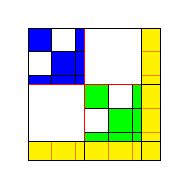
\begin{tikzpicture}[scale=1.2]
      \draw[fill=blue,draw] (0,0) -- (0,-0.25) -- (0.25,-0.25) -- (0.25,0) -- cycle; 
      \draw[fill=blue,draw] (0.25,-0.25) -- (0.25,-0.5) -- (0.5,-0.5) -- (0.5,-0.25) -- cycle; 
      \draw[fill=blue,draw] (0.5,-0.5) -- (0.5,-0.6) -- (0.6,-0.6) -- (0.6,-0.5) -- cycle;
      \draw[fill=blue,draw] (0.5,0) -- (0.5,-0.25) -- (0.6,-0.25) -- (0.6,0.) -- cycle; 
      \draw[fill=blue,draw] (0.5,-0.25) -- (0.5,-0.5) -- (0.6,-0.5) -- (0.6,-0.25) -- cycle;
      \draw[fill=blue,draw] (0.,-0.5) -- (0.,-0.6) -- (0.25,-0.6) -- (0.25,-0.5) -- cycle;
      \draw[fill=blue,draw] (0.25,-0.5) -- (0.25,-0.6) -- (0.5,-0.6) -- (0.5,-0.5) -- cycle;
      \draw[draw=red] (0.,0.) -- (0,-0.6) -- (0.6,-0.6) -- (0.6,0.) -- cycle;

      \draw[fill=green,draw] (0.6,-0.6) -- (0.6,-0.85) -- (0.85,-0.85) -- (0.85,-0.6) -- cycle; 
      \draw[fill=green,draw] (0.85,-0.85) -- (0.85,-1.1) -- (1.1,-1.1) -- (1.1,-0.85) -- cycle; 
      \draw[fill=green,draw] (1.1,-1.1) -- (1.1,-1.2) -- (1.2,-1.2) -- (1.2,-1.1) -- cycle;
      \draw[fill=green,draw] (1.1,-0.6) -- (1.1,-0.85) -- (1.2,-0.85) -- (1.2,-0.6) -- cycle; 
      \draw[fill=green,draw] (1.1,-0.85) -- (1.1,-1.1) -- (1.2,-1.1) -- (1.2,-0.85) -- cycle;
      \draw[fill=green,draw] (0.6,-1.1) -- (0.6,-1.2) -- (0.85,-1.2) -- (0.85,-1.1) -- cycle;
      \draw[fill=green,draw] (0.85,-1.1) -- (0.85,-1.2) -- (1.1,-1.2) -- (1.1,-1.1) -- cycle;
      \draw[draw=red] (0.6,-0.6) -- (0.6,-1.2) -- (1.2,-1.2) -- (1.2,-0.6) -- cycle;

      \draw[fill=yellow,draw] (1.2,-1.2) -- (1.2,-1.4) -- (1.4,-1.4) -- (1.4,-1.2) -- cycle;
      \draw[fill=yellow,draw] (1.2,0.) -- (1.2,-0.6) -- (1.4,-0.6) -- (1.4,0.) -- cycle;
      \draw[fill=yellow,draw] (1.2,-0.6) -- (1.2,-1.2) -- (1.4,-1.2) -- (1.4,-0.6) -- cycle;
      \draw[fill=yellow,draw] (0.,-1.2) -- (0.,-1.4) -- (0.6,-1.4) -- (0.6,-1.2) -- cycle;
      \draw[fill=yellow,draw] (0.6,-1.2) -- (0.6,-1.4) -- (1.2,-1.4) -- (1.2,-1.2) -- cycle;
      \draw[draw=orange] (1.2,-0.25) -- (1.4,-0.25);
      \draw[draw=orange] (1.2,-0.5) -- (1.4,-0.5);

      \draw[draw=orange] (1.2,-0.85) -- (1.4,-0.85);
      \draw[draw=orange] (1.2,-1.1) -- (1.4,-1.1);

      \draw[draw=orange] (0.25,-1.2) -- (0.25,-1.4);
      \draw[draw=orange] (0.5,-1.2) -- (0.5,-1.4);

      \draw[draw=orange] (0.85,-1.2) -- (0.85,-1.4);
      \draw[draw=orange] (1.1,-1.2) -- (1.1,-1.4);

      \draw (0,0) -- (0,-1.4) -- (1.4,-1.4) -- (1.4,0) -- cycle;

    \end{tikzpicture}
  \end{figure}
\end{frame}

\subsection{Implicit methods}

\begin{frame}[fragile]{Principe of FETI method on two subdomains}
  \scriptsize
  \begin{block}{\small Algebraic approach}
    \begin{itemize}
      \item Same domain decomposition as Primal Schur decomposition domain :\\
      $
      \left(\begin{array}{ccc}
        A_{11} & 0 & A_{13} \\
         0 & A_{22} & A_{23} \\
         A_{31} & A_{32} & A_{33} 
      \end{array}\right) \left(\begin{array}{c}
        x_{1} \\ x_{2} \\ x_{3}
      \end{array}\right) =
      \left(\begin{array}{c}
        b_{1} \\ b_{2} \\ b_{3}
      \end{array}\right)
      $
      \item Decompose $A_{33} = A_{33}^{(1)} + A_{33}^{(2)}$ and $b_{3} = b_{3}^{(1)} + b_{3}^{(2)}$ 
      \item Equivalent linear system :
      $
      \left\{
      \begin{array}{l}
        \left(\begin{array}{cc}
          A_{11} & A_{13} \\
          A_{31} & A_{33}^{(1)}
        \end{array}\right) \left(
          \begin{array}{c} x_{1} \\ x_{3} 
          \end{array}\right) = \left(
        \begin{array}{c} 
          b_{1} \\ b_{3}^{(1)} + \left(b_{3}^{(2)} - A_{32}x_{2} -A_{33}^{(2)}x_{3}^{(2)}\right)\end{array}\right)
      \\
      \left(\begin{array}{cc}
        A_{22} & A_{23} \\
        A_{32} & A_{33}^{(2)}
      \end{array}\right) \left(
        \begin{array}{c} x_{2} \\ x_{3} 
        \end{array}\right) = \left(
      \begin{array}{c} b_{2} \\ b_{3}^{(2)} + \left(b_{3}^{(1)} - A_{31}x_{1} -A_{33}^{(1)}x_{3}^{(1)}\right)\end{array}\right)
    \end{array} 
      \right.
      $
      \item $\lambda = b_{3}^{(2)} - A_{32}x_{2} -A_{33}^{(2)}x_{3}^{(2)} = -\left(b_{3}^{(1)} - A_{31}x_{1} -A_{33}^{(1)}x_{3}^{(1)}\right)$
      \item Equivalent to find $(x_{1},x_{2},x_{3}^{(1)}, x_{3}^{(2)}, \lambda)$ verifying :
      $
      \left\{
        \begin{array}{l}
          \mathcal{A}_{i}.u_{i} = 
          \left(\begin{array}{cc}
            A_{ii} & A_{i3} \\
            A_{3i} & A_{33}^{(i)}
          \end{array}\right) \left(
          \begin{array}{c} x_{i} \\ x^{(i)}_{3} 
          \end{array}\right) = \left(
          \begin{array}{c} 
            b_{i} \\ b_{3}^{(i)} \pm \lambda
          \end{array}\right) = v_{i} \pm P_{i}^{t}.\lambda, i=1,2;\; P_{i}^{t}\mbox{ prolongement de }\Gamma_{3}\rightarrow \overline{\Omega_{i}}
          \\
          x_{3}^{(1)} = x_{3}^{(2)} \Leftrightarrow P_{1}.v_{1} = P_{2}.v_{2}; P_{i}\mbox{ restriction de }\overline{\Omega_{i}}\rightarrow \Gamma_{3}
        \end{array}
      \right.
      $
    \end{itemize}
  \end{block}
\end{frame}

\begin{frame}[fragile]{Algebraic approach of the FETI method}
  \scriptsize
  \begin{block}{\small FETI Method}
    \begin{itemize}
      \item Must solve
      $
      \left(\begin{array}{ccc}
        \mathcal{A}_{1} & 0 & P_{1}^{t} \\
        0 & \mathcal{A}_{2} & -P_{2}^{t} \\
        P_{1} & -P_{2} & 0
      \end{array}\right)
      \left(\begin{array}{c} u_{1} \\ u_{2} \\ \lambda \end{array}\right) =
      \left(\begin{array}{c} v_{1} \\ v_{2} \\ 0 \end{array}\right)
      $
      \item $u_{1}$ and $u_{2}$ could be considered as linear operator with variable $\lambda$ :
      $u_{1}(\lambda) = \mathcal{A}_{1}^{-1}\left(v_{1} - P_{1}^{t}\lambda\right)$ and
      $u_{2}(\lambda) = \mathcal{A}_{2}^{-1}\left(v_{2} + P_{2}^{t}\lambda\right)$
      \item Idea of FETI Method is to solve linear system $P_{1}.u_{1}(\lambda) -P_{2}.u_{2}(\lambda) = 0$ with an iterative method (Conjugate gradient, GMRES, and so.)
    \end{itemize}
  \end{block}

  \begin{exampleblock}{\small An iteration of iterative solver with FETI Method with two processors}
    For a processor, the matrix-vector product in FETI method is :
    \begin{itemize}
      \item Compute $f_{i} = v_{i} \mp P_{i}^{t}\lambda$
      \item Solve $\mathcal{A}_{i}.u_{i} = f_{î}$
      \item Exchange $P{i}.u_{i} = u_{i}|_{\Gamma_{3}}$ with other processor
      \item Compute $P_{1}.u_{1} - P_{2}.u_{2}$
    \end{itemize}
  \end{exampleblock}
\end{frame}

\begin{frame}[fragile]{FETI-2LM (complement)}
  \scriptsize
  \begin{block}{FETI-2LM}
  A more robust variant of FETI method :
  \begin{itemize}
    \item We take two lagragian variables instead of one lagragian variable
    $
    \left\{
      \begin{array}{l}
        \mathcal{A}_{i}.u_{i} = 
        \left(\begin{array}{cc}
          A_{ii} & A_{i3} \\
          A_{3i} & A_{33}^{(i)} + R_{33}^{(i)}
        \end{array}\right) \left(
        \begin{array}{c} x_{i} \\ x^{(i)}_{3} 
        \end{array}\right) = \left(
        \begin{array}{c} 
          b_{i} \\ b_{3}^{(i)} + \lambda^{(i)}
        \end{array}\right) = v_{i} + P_{i}^{t}.\lambda^{(i)}, i=1,2;\; P_{i}^{t}\mbox{ prolongement de }\Gamma_{3}\rightarrow \overline{\Omega_{i}}
        \\
        x_{3}^{(1)} = x_{3}^{(2)} \Leftrightarrow P_{1}.v_{1} = P_{2}.v_{2}; P_{i}\mbox{ restriction de }\overline{\Omega_{i}}\rightarrow \Gamma_{3}
      \end{array}
    \right.
    $ with $R_{33}^{(i)}$ to define.
    \item In global discrete system : $A_{31}.x_{1} + A_{32}.x_{2} + A_{33}.x_{3} = b_{3}$, so 
    $A_{31}.x_{1} + A_{32}.x_{2} + A_{33}^{(1)}.x_{3}^{(1)} + A_{33}^{(2)}.x_{3}^{(2)} = b_{3}^{(1)} + b_{3}^{(2)}$
    \item So using the last equation of local discrete problem : 
    $A_{3i}.x_{i} + A_{33}^{(i)}.x_{3}^{(i)} + R_{33}^{(i)}.x_{3}^{(i)} = b_{3}^{(i)} + \lambda^{(i)}$, we have 
    $R_{33}^{(1)}x_{3}^{(1)} + R_{33}^{(2)}.x_{3}^{(2)} = \lambda^{(1)} + \lambda^{(2)}$
    \item Using $x_{3}^{(1)} = x_{3}^{(2)}$, we   obtain :
    $
    \left\{
      \begin{array}{lcl}
        R_{33}^{(1)}.x_{3}^{(1)} + R_{33}^{(2)}.x_{3}^{(1)} & = & \lambda^{(1)} + \lambda^{(2)} \\
        R_{33}^{(1)}.x_{3}^{(2)} + R_{33}^{(2)}.x_{3}^{(2)} & = & \lambda^{(1)} + \lambda^{(2)}
      \end{array}
    \right.
    $
    \item Relation between $\lambda_{i}$ and $x_{3}^{(i)}$ can be explicitly computed :
      $\left(A_{33}^{(i)} - A_{3i}A_{ii}^{-1}A_{i3} + R_{33}^{(i)}\right)x_{3}^{(i)} = \lambda^{(i)} + b_{3}^{(i)} - A_{3i}A_{ii}^{-1}b_{i}$
  \end{itemize}
  \end{block}
\end{frame}

\begin{frame}[fragile]{FETI-2LM...}
  \scriptsize
  \begin{block}{FETI-2LM (continued)}
    \begin{itemize}
      \item Denote the schur complement $S^{(i)} = A_{33}^{(i)} - A_{3i}.A_{ii}^{-1}.A_{i3}$, and the condensed right-hand side 
      $c_{3}^{(i)} = b_{3}^{(i)} - A_{3i}.A_{ii}^{-1}.b_{i}$.
      \item Replace $x_{3}^{(1)}$ and $x_{3}^{(2)}$ by their values as function of $\lambda^{(1)}$ and $\lambda^{(2)}$ :
      $
      \left(\begin{array}{cc}
        I & I - (R_{33}^{(1)}+R_{33}^{(2)})(S^{(2)}+R_{33}^{(2)})^{-1} \\
        I - (R_{33}^{(1)}+R_{33}^{(2)})(S^{(1)}+R_{33}^{(1)})^{-1} & I
      \end{array}\right)
      \left(\begin{array}{c}
        \lambda^{(1)} \\ \lambda^{(2)}
      \end{array}\right) = 
      \left(\begin{array}{c}
        (S^{(2)}+R_{33}^{(2)})^{-1}c_{3}^{(2)}\\
        (S^{(1)}+R_{33}^{(1)})^{-1}c_{3}^{(1)}
      \end{array}\right)
      $
      \item "Best choice" for $R_{33}^{(1)}$ and $R_{33}^{(2)}$ : $R_{33}^{(1)} = S^{(2)}$ and $R_{33}^{(2)} = S^{(1)}$ but too expensive to compute
      \item Try to build a sparse approximation of $S^{(i)}$ for $R_{33}^{(i)}$.
    \end{itemize}
  \end{block}
\end{frame}
\end{document}
